\documentclass{article}\usepackage[]{graphicx}\usepackage[]{xcolor}
% maxwidth is the original width if it is less than linewidth
% otherwise use linewidth (to make sure the graphics do not exceed the margin)
\makeatletter
\def\maxwidth{ %
  \ifdim\Gin@nat@width>\linewidth
    \linewidth
  \else
    \Gin@nat@width
  \fi
}
\makeatother

\definecolor{fgcolor}{rgb}{0.345, 0.345, 0.345}
\newcommand{\hlnum}[1]{\textcolor[rgb]{0.686,0.059,0.569}{#1}}%
\newcommand{\hlstr}[1]{\textcolor[rgb]{0.192,0.494,0.8}{#1}}%
\newcommand{\hlcom}[1]{\textcolor[rgb]{0.678,0.584,0.686}{\textit{#1}}}%
\newcommand{\hlopt}[1]{\textcolor[rgb]{0,0,0}{#1}}%
\newcommand{\hlstd}[1]{\textcolor[rgb]{0.345,0.345,0.345}{#1}}%
\newcommand{\hlkwa}[1]{\textcolor[rgb]{0.161,0.373,0.58}{\textbf{#1}}}%
\newcommand{\hlkwb}[1]{\textcolor[rgb]{0.69,0.353,0.396}{#1}}%
\newcommand{\hlkwc}[1]{\textcolor[rgb]{0.333,0.667,0.333}{#1}}%
\newcommand{\hlkwd}[1]{\textcolor[rgb]{0.737,0.353,0.396}{\textbf{#1}}}%
\let\hlipl\hlkwb

\usepackage{framed}
\makeatletter
\newenvironment{kframe}{%
 \def\at@end@of@kframe{}%
 \ifinner\ifhmode%
  \def\at@end@of@kframe{\end{minipage}}%
  \begin{minipage}{\columnwidth}%
 \fi\fi%
 \def\FrameCommand##1{\hskip\@totalleftmargin \hskip-\fboxsep
 \colorbox{shadecolor}{##1}\hskip-\fboxsep
     % There is no \\@totalrightmargin, so:
     \hskip-\linewidth \hskip-\@totalleftmargin \hskip\columnwidth}%
 \MakeFramed {\advance\hsize-\width
   \@totalleftmargin\z@ \linewidth\hsize
   \@setminipage}}%
 {\par\unskip\endMakeFramed%
 \at@end@of@kframe}
\makeatother

\definecolor{shadecolor}{rgb}{.97, .97, .97}
\definecolor{messagecolor}{rgb}{0, 0, 0}
\definecolor{warningcolor}{rgb}{1, 0, 1}
\definecolor{errorcolor}{rgb}{1, 0, 0}
\newenvironment{knitrout}{}{} % an empty environment to be redefined in TeX

\usepackage{alltt}
\usepackage{hyperref}
\usepackage{blindtext}
\usepackage{graphicx}
\usepackage{float}
\usepackage{listings}
\usepackage{appendix}
\usepackage{amsmath}
\usepackage{comment}
\usepackage{natbib}
\usepackage[a4paper, total={6in, 8in}]{geometry}
\IfFileExists{upquote.sty}{\usepackage{upquote}}{}
\begin{document}




\subsection{Datasets}
\noindent
\textbf{Statistical GIS Boundary Files for London}: This file, offered by Greater London Autority (GLA) and available at \href{https://data.london.gov.uk/dataset/statistical-gis-boundary-files-london}{London Datastore}, provided a range of key GIS boundary files for ESRI and Map Info covering Greater London, including shape files of London Wards and London Boroughs. This data set includes Name: Name of ward, District: Name of borough, Geometry: Pair of longitude and latitude.\\

\noindent
\textbf{Crime levels by borough}: This data set, offered by Metropolitan Police Service and available at \href{https://data.london.gov.uk/dataset/recorded_crime_summary}{London Datastore}, counted the number of crimes at three different geographic levels of London (borough, ward, LSOA) per month, according to crime type from 2010 to 2021. This data set contain variables like LookUp\_BoroughName: Name of Borough and X201004: count of crimes during April 2010.\\

\noindent
\textbf{Population by Ward and Borough}: This file, offered by Greater London Autority (GLA) and available at \href{https://data.london.gov.uk/dataset/land-area-and-population-density-ward-and-borough}{London Datastore}, provided population for 2001 to 2050 for London wards and boroughs. This data set includes variables like Name: Borough name, Year: population of the year, Population: population of the borough at that year.\\

\noindent
\textbf{Trees}: The trees dataset, available as a built-in dataset in R, offers measurements from 31 felled black cherry trees and provides insights into the relationship between a tree's girth, its height, and the volume of timber it can produce. The dataset contains 3 variables: Girth: The diameter of the tree, Height: The height of the tree, Volume: The volume of timber that the tree can produce.\\

\subsection{Network Graphs}

\textbf{Definition and Utility:}
Network graphs, often referred to as graphs or networks, are a powerful data visualisation method used to depict relationships between entities. These entities, known as nodes, are interconnected by edges or links, which represent relationships, connections, or interactions. Network graphs find extensive utility in various fields, such as social network analysis, transportation systems, and even biological networks like protein-protein interactions. They excel at revealing complex dependencies and structures, making them a critical tool for understanding relational data.

\subsubsection{The Mathematics behind Network Graphs:}
Constructing network graphs involves several mathematical intricacies. Here we present just a few of the many concepts that play a role in the creation of such graphs:

\begin{enumerate}
\item \textbf{Nodes and Edges}: Mathematically, a network graph, \(G\), is defined as \(G = (V, E)\), where \(V\) represents the set of nodes and \(E\) represents the set of edges connecting these nodes.
\item \textbf{Node Degree}: The degree of a node is the number of edges connected to it. In a directed graph, nodes can have both in-degrees and out-degrees.
\item \textbf{Centrality Measures}: Centrality metrics like degree centrality, betweenness centrality, and closeness centrality provide insights into the relative importance or influence of nodes within a network.
\item \textbf{Graph Metrics}: Graph theory concepts like shortest paths, connected components, and clustering coefficients are used toanalyse the network's structure.
\end{enumerate}

\noindent
\textbf{Formulas used in Network Graphs:}

\begin{enumerate}
\item \textbf{Degree of a Node (Undirected Graph)}:
\[
\text{Degree}(v) = \sum_{w \in V} A(v, w)
\]
where \(A(v, w)\) is the adjacency matrix element, indicating whether there is a connection between nodes \(v\) and \(w\).
\item \textbf{Degree of a Node (Directed Graph)}:
\[
\text{In-Degree}(v) = \sum_{w \in V} A(w, v)
\]
\[
\text{Out-Degree}(v) = \sum_{w \in V} A(v, w)
\]
\item \textbf{Betweenness Centrality (for unweighted graphs)}:
\[
C_B(v) = \sum_{s \neq v \neq t} \frac{\sigma_{st}(v)}{\sigma_{st}}
\]
where \(\sigma_{st}\) is the number of shortest paths from node \(s\) to \(t\), and \(\sigma_{st}(v)\) is the number of those paths passing through node \(v\).
\end{enumerate}

\subsubsection{Network Graphs in Practice}




\begin{figure}[h]
\centering
\begin{knitrout}\scriptsize
\definecolor{shadecolor}{rgb}{0.969, 0.969, 0.969}\color{fgcolor}\begin{kframe}
\begin{alltt}
\hlcom{# Plot the graph}
\hlcom{#plot(lesmis_graph, layout = layout, vertex.label.cex = 0.7, main = "Character Interactions in Les Misérables")}
\end{alltt}
\end{kframe}
\end{knitrout}
\end{figure}
d
\subsection{Geographic Maps and Spatial Data Visualisation}

A \textbf{geographical maps} is a visual representation of an area—a symbolic depiction highlighting relationships between elements of that space, such as objects, regions, or themes. Maps have been used for centuries to navigate and explore the world, and they play a crucial role in understanding our environment, both locally and globally. These maps serve as canvases on which spatial data is painted, allowing for a visual comprehension of information that might otherwise remain abstract.\\

\noindent
Before moving on to the spatial data visualisation. It is essential to understand how we map the the earth on a plane. The Earth, a three-dimensional spheroid, can be transformed on a plane through map projections. Each projection offers a different way to "flatten" the Earth, and as a result, each has its strengths and distortions. For instance, the Mercator projection preserves angles but distorts areas as you move towards the poles. Beyond projections, coordinate systems, like the commonly used latitude and longitude, provide a standardized way to pinpoint any location on Earth.

\begin{itemize}
\item \textbf{Latitude} measures the angle between a point on the Earth's surface and the equator, moving north or south. And latitude values range from -90 degrees (South Pole) to +90 degrees (North Pole). The equator, which divides the Earth into the Northern and Southern Hemispheres, is at 0 degree latitude.
\item \textbf{Longitude} measures the angle between a point on the Earth's surface and the prime meridian, moving east or west.
And longitude values range from -180 degrees to +180 degrees. The prime meridian, which is at 0 degree longitude, runs from the North Pole through Greenwich, England, to the South Pole. It divides the Earth into the Eastern and Western Hemispheres.
\end{itemize}

\noindent
Together, lines of longitude and latitude create a grid system over the Earth's surface. By providing both a latitude and longitude value, one can specify an exact location on the Earth's surface. For example, the coordinates (0° N, 0° E) would indicate the intersection of the equator and the prime meridian, located in the Gulf of Guinea off the west coast of Africa.\\

\noindent
\textbf{Spatial data visualisation}\\

\noindent
Spatial data visualisation are powerful tools that transform raw, often complex datasets into visual representations, revealing patterns, relationships, and insights rooted in location. At their core, maps provide a spatial context, allowing us to see the world's intricate web of interconnectedness. Today, with the surge in big data and advanced visualisation tools, spatial data visualisation is not just about presenting information but also about telling compelling stories, guiding decision-making, and predicting future trends based on geographical patterns.



\noindent
Here, we are going to construct a geographical map of the Greater London and show each ward. 

\begingroup
\setlength{\intextsep}{5pt plus 2pt minus 2pt}
\setlength{\textfloatsep}{5pt plus 2pt minus 2pt}
\setlength{\abovecaptionskip}{2pt plus 1pt minus 1pt}
\setlength{\belowcaptionskip}{2pt plus 1pt minus 1pt}

\begin{figure}[H]
\begin{knitrout}\scriptsize
\definecolor{shadecolor}{rgb}{0.969, 0.969, 0.969}\color{fgcolor}\begin{kframe}
\begin{alltt}
\hlcom{# Plot London map by ward}
\hlkwd{ggplot}\hlstd{(}\hlkwc{data} \hlstd{= london_boroughs)} \hlopt{+} \hlkwd{geom_sf}\hlstd{(}\hlkwc{fill} \hlstd{=} \hlstr{"lightblue"}\hlstd{,} \hlkwc{color} \hlstd{=} \hlstr{"black"}\hlstd{)} \hlopt{+}
  \hlkwd{theme_minimal}\hlstd{()} \hlopt{+} \hlkwd{labs}\hlstd{(}\hlkwc{y}\hlstd{=}\hlstr{"Latitude"}\hlstd{,} \hlkwc{x}\hlstd{=}\hlstr{"Longitude"}\hlstd{)}
\end{alltt}
\end{kframe}

{\centering 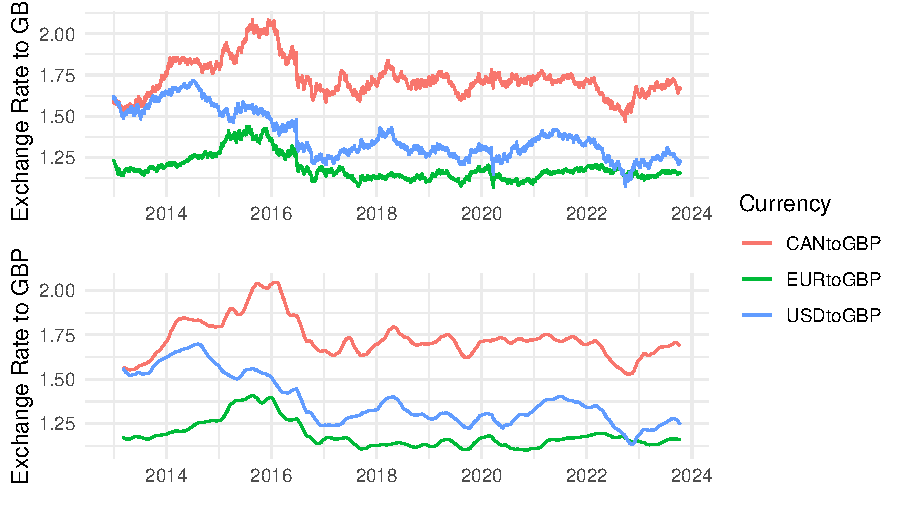
\includegraphics[width=\maxwidth]{figure/beamer-unnamed-chunk-2-1} 

}


\end{knitrout}
\centering
\caption{London Wards Map}
\label{fig:London Wards Map}
\end{figure}
\endgroup

\noindent
From Figure~\ref{fig:London Wards Map}, we are introduced to a detailed layout of all wards within Greater London, pinpointed by their geographical coordinates. While this map provides a clear depiction of location and boundaries, it offers limited insight into the dynamics of crime distribution.\\

\noindent
Hence, we will use a more informativevisualisation: a choropleth map showcasing crime rates by borough. Here, crime rates are calculated by dividing the total crime count in each borough by its respective population as of 2020. This per capita approach normalizes the data, ensuring comparability across boroughs with different population sizes.

\begin{figure}[H]
\begin{knitrout}\scriptsize
\definecolor{shadecolor}{rgb}{0.969, 0.969, 0.969}\color{fgcolor}\begin{kframe}
\begin{alltt}
\hlcom{# Plot the Crime rate in London by boroughs}
\hlkwd{ggplot}\hlstd{(}\hlkwc{data}\hlstd{=aggregated_data)} \hlopt{+} \hlkwd{geom_sf}\hlstd{(}\hlkwd{aes}\hlstd{(}\hlkwc{fill}\hlstd{=Crime_rate))} \hlopt{+}
  \hlkwd{geom_sf_text}\hlstd{(}\hlkwd{aes}\hlstd{(}\hlkwc{label} \hlstd{= DISTRICT,} \hlkwc{geometry} \hlstd{= centroid),}
               \hlkwc{size} \hlstd{=} \hlnum{2.5}\hlstd{,} \hlkwc{check_overlap} \hlstd{=} \hlnum{TRUE}\hlstd{)} \hlopt{+}
  \hlkwd{scale_fill_gradient}\hlstd{(}\hlkwc{low}\hlstd{=}\hlstr{"Green"}\hlstd{,} \hlkwc{high}\hlstd{=}\hlstr{"red"}\hlstd{)} \hlopt{+} \hlkwd{theme_minimal}\hlstd{()} \hlopt{+}
  \hlkwd{labs}\hlstd{(}\hlkwc{fill}\hlstd{=}\hlstr{"Crime rate"}\hlstd{)}
\end{alltt}
\end{kframe}

{\centering 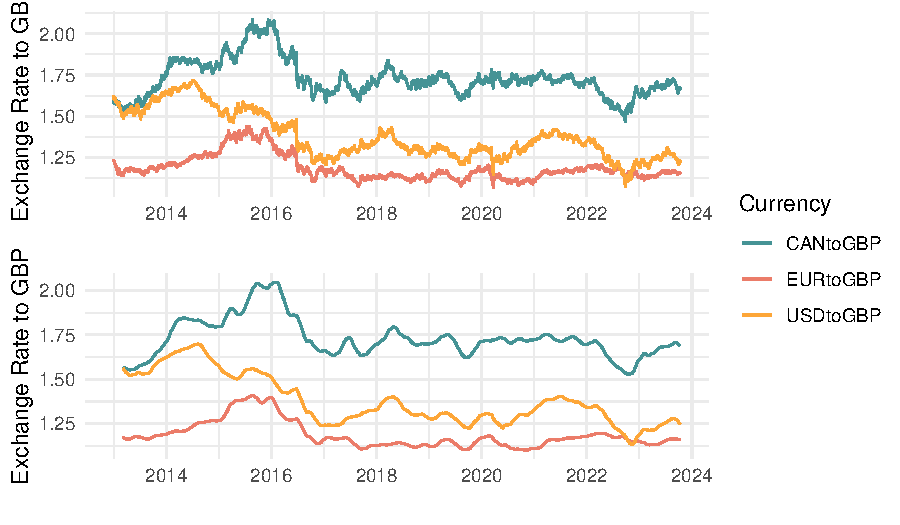
\includegraphics[width=\maxwidth]{figure/beamer-unnamed-chunk-3-1} 

}


\end{knitrout}
\centering
\caption{Crime rate by boroughs in London in 2020}
\label{fig:crime rate london}
\end{figure}

\noindent
From Figure~\ref{fig:crime rate london}, Westminster stands out, labeled in red, indicating a higher crime rate. This visual marker highlights Westminster as an area of particular concern regarding criminal activity. This could be attributed to factors like its status as a central, densely populated area with significant tourist traffic and commercial activity, which often correlate with higher crime rates.\\

\noindent
In contrast, the map reveals a trend where rural or less densely populated areas tend to be safer, as evidenced by their lighter coloration. These areas typically experience lower crime rates, possibly due to factors such as smaller populations, less anonymity for potential offenders, and different socio-economic dynamics compared to urban centers.\\

\noindent
The choropleth map of London’s crime rates elucidates key spatial patterns in crime distribution. It highlights the variance in crime rates from urban centers to rural areas, accentuating the higher crime rates in central, densely populated areas like Westminster, depicted in red, compared to the lighter shades marking safer, rural boroughs. This visual tool facilitates an understanding of how urbanization, socio-economic status, and population density impact crime rates across the boroughs.

\subsection{3D and Interactive Visualisations}

ggplot2 is one of the most popular data visualisation libraries in R, but it is primarily designed for 2D data visualisation. Directly creating 3D views with ggplot2 can be challenging.\\

\noindent
R provides several packages for 3Dvisualisation, such as rgl, plot3D, rayshader, and others, which are specifically designed for three-dimensional data. These packages offer the capability to create 3D scatter plots, surface plots, heat maps, contour maps, and more.\\

\noindent
\textbt{rgl}: This is one of the most popular R packages for creating interactive 3D charts. It supports various types of 3D graphics including points, lines, and surfaces, and allows users to interactively rotate, zoom, and pan the view.\\
\textbt{scatterplot}:This package provides a function to create 3D scatter plots. It does not support interactive manipulation, but the generated graphics are well-suited for display in static reports.\\

\noindent
3D data visualisation is an approach that employs three-dimensional graphics to represent complex data structures, allowing for an immersive exploration of information. Unlike traditional 2D visualisations (like bar graphs or line charts), 3D visualisations can convey an additional dimension of data, making them particularly valuable in specific contexts.\\

\noindent
Our first example will be  a scatter plot. We can use scatterplot3d package to help us for data visualisation.

\begin{knitrout}\scriptsize
\definecolor{shadecolor}{rgb}{0.969, 0.969, 0.969}\color{fgcolor}\begin{kframe}
\begin{alltt}
\hlcom{# Generate colors based on the Volume variable}
\hlstd{colors} \hlkwb{<-} \hlkwd{colorRampPalette}\hlstd{(}\hlkwd{c}\hlstd{(}\hlstr{"blue"}\hlstd{,} \hlstr{"red"}\hlstd{))(}\hlkwd{length}\hlstd{(}\hlkwd{unique}\hlstd{(trees}\hlopt{$}\hlstd{Volume)))}
\hlstd{color_assign} \hlkwb{<-} \hlstd{colors[}\hlkwd{as.numeric}\hlstd{(}\hlkwd{as.factor}\hlstd{(trees}\hlopt{$}\hlstd{Volume))]}
\hlcom{# Create 3d scatter plot with colors}
\hlkwd{scatterplot3d}\hlstd{(trees}\hlopt{$}\hlstd{Girth, trees}\hlopt{$}\hlstd{Height, trees}\hlopt{$}\hlstd{Volume,}
              \hlkwc{color}\hlstd{=color_assign,}
              \hlkwc{main}\hlstd{=}\hlstr{"3D Scatterplot of trees data"}\hlstd{,}
              \hlkwc{xlab}\hlstd{=}\hlstr{"Girth (inches)"}\hlstd{,}
              \hlkwc{ylab}\hlstd{=}\hlstr{"Height (ft)"}\hlstd{,}
              \hlkwc{zlab}\hlstd{=}\hlstr{"Volume (cubic ft)"}\hlstd{)}
\end{alltt}
\end{kframe}\begin{figure}[H]

{\centering 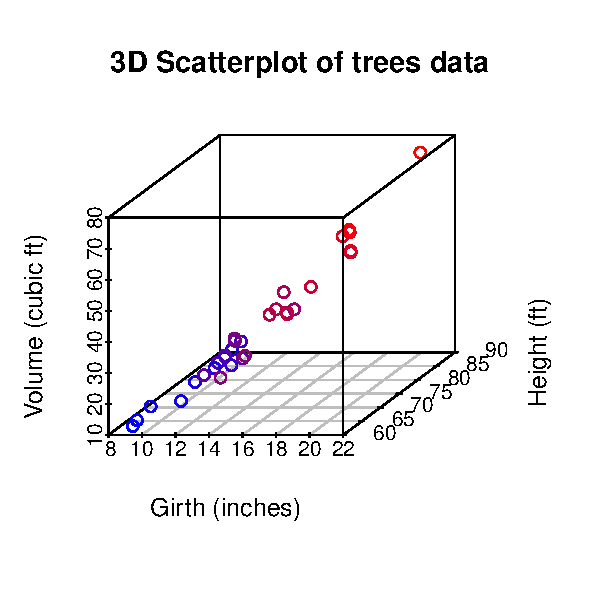
\includegraphics[width=\maxwidth]{figure/beamer-3d1-1} 

}

\caption[3d scatter plot]{3d scatter plot}\label{fig:3d1}
\end{figure}

\end{knitrout}


\section{Trees Dataset in R}
XXX
\subsection{Advanced Visualisation Techniques}
XXX
\section{Practical Implementations}
XXX
\section{Case Studies}
\subsection{Market Analysis Dashboards}
XXX
\subsection{Healthcare Data Visualisation}
XXX
\section{State-of-the-Art Approaches}
XXX
\section{Conclusion}
XXX


\end{document}
